\section{Evaluation Methodology: LAFC-Evict Construction}
\label{sec:benchmark-design}

This section defines the scientific abstraction underlying \lafc\ before
describing how it is packaged for release (the end-to-end pipeline is
summarized in Figure~\ref{fig:pipeline}). A \emph{trace} is a sequence of
\emph{requests} (accesses) to objects. A \emph{cache state} is the set of
objects resident in a bounded-capacity cache at a point in the trace. When
a request misses and the cache is full, the system faces an
\emph{eviction decision}: choose one resident object, a \emph{candidate
victim}, to evict before admitting the requested object. \lafc\ treats
every such decision, across every trace, capacity, and horizon evaluated,
as one supervised unit; Section~\ref{sec:label-generation} defines the exact
formal quantities (finite-horizon counterfactual loss, optimal candidate
set, regret) built on top of this abstraction, following directly from the
worked example in Section~\ref{sec:background}.

The cache abstraction used throughout this paper is intentionally narrow
and stated explicitly here rather than left implicit: objects are
unit-sized (no byte-weighted or variable-size accounting), capacity is
counted in objects, and admission of the requested object is
unconditional (eviction is never avoided by refusing admission).
Section~\ref{sec:limitations} discusses the consequences of this scope
boundary; every claim in this paper should be read as bounded by it.

\begin{figure}[t]
  \centering
  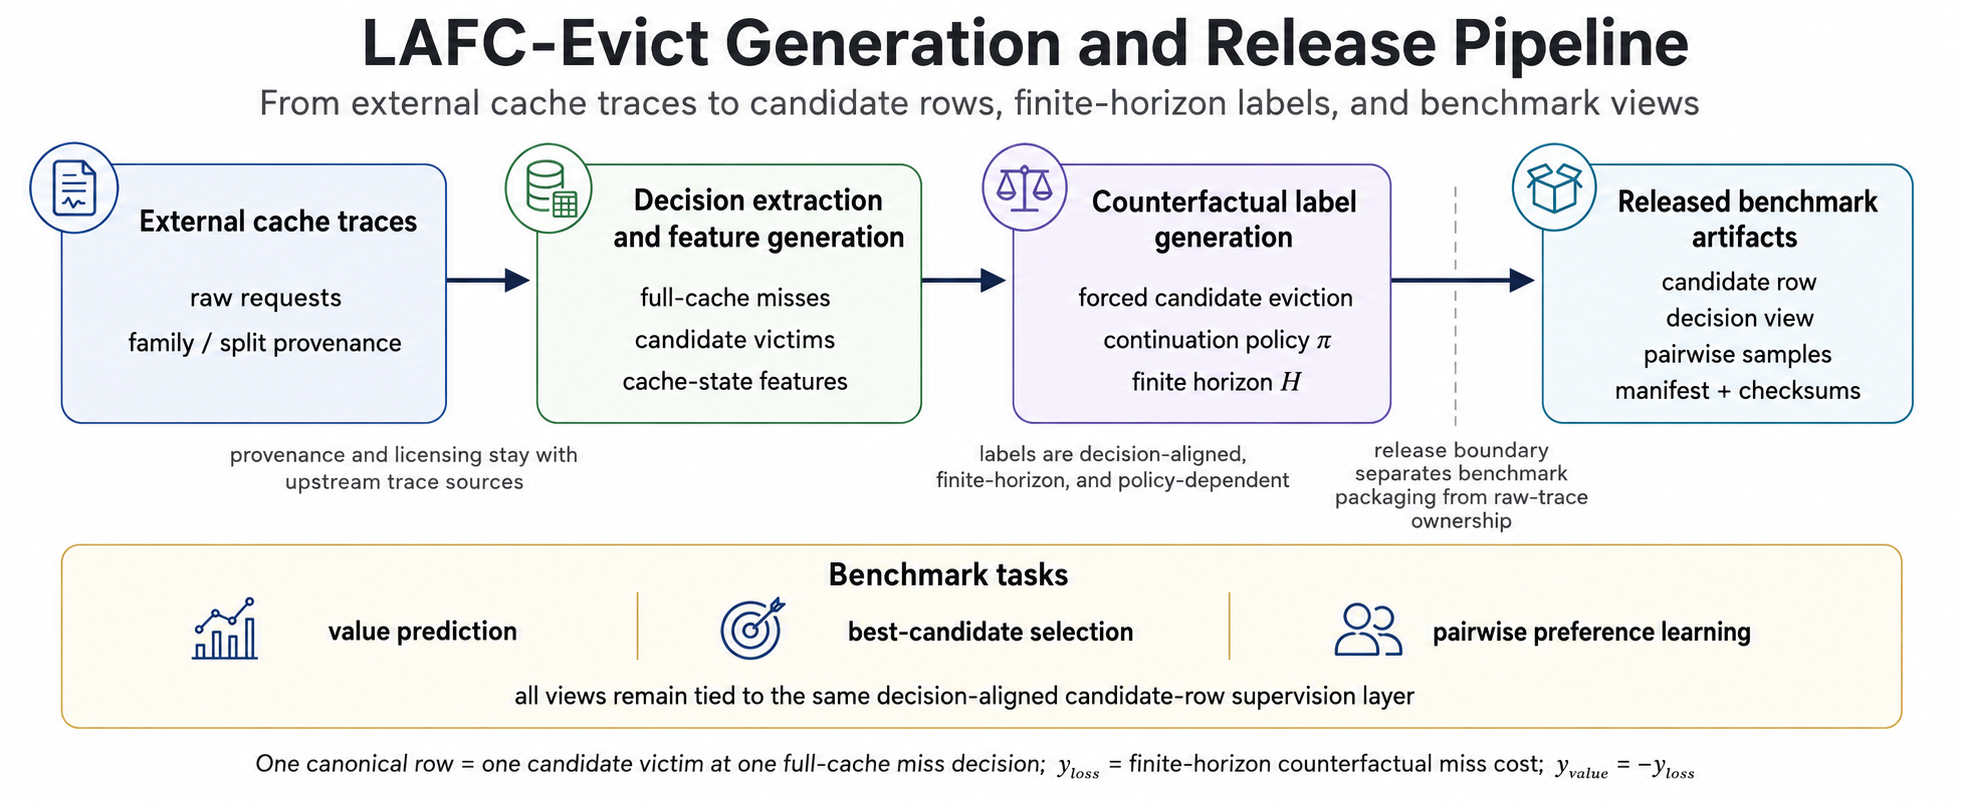
\includegraphics[width=\textwidth]{../../64BDAA68-CBD4-4E8E-800B-467D62C0D9DE.png}
  \caption{LAFC-Evict generation and release pipeline. External cache traces are converted into decision-level candidate rows, finite-horizon counterfactual labels, and released benchmark views for value prediction, best-candidate selection, and pairwise preference learning.}
  \label{fig:pipeline}
\end{figure}

The evaluated dataset covers five trace families -- \texttt{cloudphysics}\footnote{\texttt{cloudphysics} is a historical internal family identifier retained in project manifests, evidence records, and code for reproducibility. The underlying workload is Alibaba Cloud's Elastic Block Storage production block-storage trace, not the VMware/CloudPhysics dataset. Reader-facing prose below refers to this workload as ``alibaba-block.''},
\texttt{metacdn}, \texttt{metakv}, \texttt{twemcache}, and
\texttt{wiki2018} -- chosen to span a CDN workload, a key-value workload,
two additional production-derived workloads, and one intentionally
included negative/control workload (wiki2018; Sections~\ref{sec:characterization}
and~\ref{sec:mechanisms} show why it degenerates and treat that as a
useful, explained result rather than a benchmark defect). Two further
families, \texttt{brightkite} and \texttt{citibike}, are excluded from the
open release subset for redistribution reasons; this is a release-packaging
boundary, not a claim that the underlying generated corpus is limited to
five families. This five-family evaluated corpus is itself broader than
the currently downloadable public v0.3 subset, which packages only the
wiki2018 slice; the Data Availability statement details the redistribution
clearance and hosting status of the other four evaluated families. Not
every family appears in every split (e.g.\ metacdn
contributes train/validation but no test decisions); split assignment is
produced upstream of this release package and is normalized and validated,
not assigned, here.

The evaluation in this paper is organized to satisfy four requirements:
\begin{enumerate}[leftmargin=*]
  \item \textbf{Decision alignment.} Preserve within-decision candidate
  competition rather than treating candidates as i.i.d.\ points.
  \item \textbf{Task multiplicity.} Support pointwise (candidate-level),
  decision-level, and pairwise views of the same underlying supervision.
  \item \textbf{Closed-loop grounding.} Evaluate the offline labels
  against actual closed-loop cache-policy behavior rather than presenting
  them as self-validating (Sections~\ref{sec:closed-loop}
  and~\ref{sec:linkage}).
  \item \textbf{Reproducibility.} Expose validated, checksummed evidence
  for every reported number (Section~\ref{sec:release-validation}).
\end{enumerate}

\begin{table}[tbp]
  \centering
  \small
  \caption{Canonical evaluation protocol and workload specifications per trace family. Every family has release capacities of $\{32, 64, 128, 256\}$ and horizons of $\{4, 8, 16\}$, while closed-loop evaluation focuses on capacities $\{32, 128\}$.}
  \label{tab:evaluation-protocols}
  \begin{tabularx}{\textwidth}{@{}l P{0.13\textwidth} c c L c@{}}
    \toprule
    Family & Workload & Splits & CL Split & Scored Window & Warm-up / Init \\
    \midrule
    \texttt{alibaba-block} & Block Storage & train/val/test & test & 2 chunks (8,192 req.) & Warm \\
    \texttt{metacdn} & CDN Cache & train/val & validation & 3 chunks (20,480 req.) & Warm \\
    \texttt{metakv} & Key-Value & train/val/test & test & 1 chunk (4,096 req.) & Cold Start \\
    \texttt{twemcache} & Memcached & train/val/test & test & 2 chunks (8,192 req.) & Warm \\
    \texttt{wiki2018} & Wikipedia & train/val/test & test & 1 chunk (4,096 req.) & Warm \\
    \bottomrule
  \end{tabularx}
\end{table}


The canonical workload and evaluation parameters are summarized in Table~\ref{tab:evaluation-protocols}. When reading and interpreting the results, the following trace-specific design nuances should be kept in mind:
\begin{itemize}[leftmargin=*]
  \item \textbf{MetaCDN Validation Status:} Tier-1 closed-loop evidence for MetaCDN uses validation-window chunks because no Tier-1 test-split chunks are available at these capacities. The separate learned-policy campaign evaluates MetaCDN under its own independent held-out protocol.
  \item \textbf{MetaKV Cold Start:} MetaKV is evaluated starting from an empty cache (a cold start) with no leading unscored warm-up, whereas the other four workload families continuous-warmup from preceding unscored trace prefixes.
  \item \textbf{Wiki2018 Negative Control:} Wiki2018 is a deterministic zero-reuse negative-control workload where all candidate eviction options result in identical miss costs (100\% tie-degenerate, zero random regret), acting as a baseline verification of cache boundaries.
\end{itemize}

Detailed release characteristics, including candidate scale (277M rows) and exact split breakdowns, are provided in Appendix~\ref{sec:appendix-release-tables} (Tables~\ref{tab:dataset-scale} and~\ref{tab:split-counts}).
